\documentclass[12pt,a4paper,oneside]{report}
\usepackage[T1]{fontenc}
\usepackage[utf8]{inputenc}
\usepackage{mathptmx}
\usepackage{microtype}
\usepackage[a4paper,left=1.25in,right=1in,top=1in,bottom=1in]{geometry}
\usepackage{setspace}
\usepackage{graphicx}
\usepackage{amsmath}
\usepackage{array,tabularx,longtable,multirow}
\usepackage[table]{xcolor}
\usepackage{enumitem}
\usepackage{caption}
\usepackage{titlesec}
\usepackage{tocloft}
\usepackage{listings}
\usepackage{tikz}
\usetikzlibrary{positioning,arrows.meta,shapes.geometric,fit,calc}
\usepackage{pgfplots}
\pgfplotsset{compat=1.17}
\usepackage{url}
\usepackage[hidelinks]{hyperref}

\onehalfspacing
\setlength{\emergencystretch}{3em}
\setlength{\parindent}{0.5in}
\setlength{\parskip}{4pt}

% Captions: "Fig 1.1:" and "Table 1.1:" in bold
\DeclareCaptionLabelFormat{figlab}{Fig #2}
\captionsetup[figure]{labelformat=figlab,labelsep=colon,labelfont=bf,font=small,justification=centering}
\captionsetup[table]{labelsep=colon,labelfont=bf,font=small,justification=centering,skip=4pt}

% Chapter heading: CHAPTER n, title in capitals, centred
\titleformat{\chapter}[display]{\normalfont\bfseries\Large\centering}{CHAPTER \thechapter}{8pt}{\MakeUppercase}
\titlespacing*{\chapter}{0pt}{-20pt}{20pt}
\titleformat{\section}{\normalfont\bfseries\large}{\thesection}{0.6em}{}
\titleformat{\subsection}{\normalfont\bfseries\normalsize}{\thesubsection}{0.6em}{\MakeUppercase}

% Table of contents and lists
\renewcommand{\contentsname}{\centering TABLE OF CONTENTS}
\renewcommand{\listfigurename}{\centering LIST OF FIGURES}
\renewcommand{\listtablename}{\centering LIST OF TABLES}
\renewcommand{\cfttoctitlefont}{\hfill\Large\bfseries}
\renewcommand{\cftaftertoctitle}{\hfill}
\renewcommand{\cftloftitlefont}{\hfill\Large\bfseries}
\renewcommand{\cftafterloftitle}{\hfill}
\renewcommand{\cftlottitlefont}{\hfill\Large\bfseries}
\renewcommand{\cftafterlottitle}{\hfill}
\renewcommand{\cftchapfont}{\bfseries}
\renewcommand{\cftchappagefont}{\bfseries}
\renewcommand{\cftchapleader}{\cftdotfill{\cftdotsep}}
\renewcommand{\cftchappresnum}{}
\setlength{\cftbeforechapskip}{6pt}
\renewcommand{\cftfigpresnum}{}
\renewcommand{\cfttabpresnum}{}
\setlength{\cftfignumwidth}{2.4em}
\setlength{\cfttabnumwidth}{2.4em}
\renewcommand{\thefigure}{\thechapter.\arabic{figure}}
\renewcommand{\thetable}{\thechapter.\arabic{table}}

% Tables: grey header row
\definecolor{hdr}{gray}{0.85}
\newcommand{\hrow}{\rowcolor{hdr}}
\newcolumntype{L}{>{\raggedright\arraybackslash}X}
\renewcommand{\arraystretch}{1.2}

% Code listings
\lstset{basicstyle=\ttfamily\scriptsize,breaklines=true,frame=single,columns=fullflexible,
  keywordstyle=\bfseries,showstringspaces=false,numbers=left,numberstyle=\tiny,xleftmargin=1.5em,
  language=Python,upquote=true}
\renewcommand{\lstlistingname}{Listing}

\newcommand{\cls}[1]{\textsc{#1}}

\begin{document}

% ---------------- Cover ----------------
\begin{titlepage}
\centering
\vspace*{-0.3in}
{\LARGE\bfseries\setstretch{1.25}
AGENTIC PILOT: AN EVIDENCE-DRIVEN LOCAL AUTONOMOUS AI AGENT FRAMEWORK FOR PRIVACY-PRESERVING INTELLIGENT TASK AUTOMATION\par}
\vspace{0.12in}
{\large\bfseries A CASE STUDY REPORT\par}
\vspace{0.08in}
{\large\itshape Submitted by\par}
\vspace{0.05in}
{\Large\bfseries SUDESH P [RA2512005010025]\par}
\vspace{0.08in}
{\large\itshape Under the Guidance of\par}
\vspace{0.05in}
{\Large\bfseries Dr. KANCHANA M\par}
{\normalsize (Professor, Department of Computing Technologies)\par}
\vspace{0.08in}
{\large\itshape in partial fulfilment of the requirements for the course\par}
\vspace{0.05in}
{\large\bfseries 21CSC601T - CASE STUDY\par}
\vspace{0.12in}
{\Large\bfseries MASTER OF TECHNOLOGY\par}
{\large in\par}
{\Large\bfseries COMPUTER SCIENCE ENGINEERING\par}
\vspace{0.12in}

\includegraphics[width=2.2in]{fig/srm_logo.jpg}\par
\vspace{0.12in}
{\large\bfseries\setstretch{1.25}
DEPARTMENT OF COMPUTING TECHNOLOGIES\\
COLLEGE OF ENGINEERING AND TECHNOLOGY\\
SRM INSTITUTE OF SCIENCE AND TECHNOLOGY\\
KATTANKULATHUR - 603 203\par}
\vspace{0.15in}
{\normalsize\bfseries NOVEMBER 2026\par}
\end{titlepage}

\pagenumbering{roman}
\setcounter{page}{2}

% ---------------- Bonafide ----------------
\begin{center}
{\bfseries SRM INSTITUTE OF SCIENCE AND TECHNOLOGY\\ KATTANKULATHUR - 603 203\par}
\vspace{0.4in}
{\bfseries\large BONAFIDE CERTIFICATE\par}
\end{center}
\vspace{0.2in}
\noindent Certified that 21CSC601T - Case Study report titled ``\textbf{Agentic Pilot: An Evidence-Driven Local Autonomous AI Agent Framework for Privacy-Preserving Intelligent Task Automation}'' is the bonafide work of \textbf{SUDESH P [RA2512005010025]} who carried out the case study under my supervision. Certified further, that to the best of my knowledge the work reported herein does not form any other project report or dissertation on the basis of which a degree or award was conferred on an earlier occasion on this or any other candidate.

\vspace{1.8in}
\noindent
\begin{tabular}{@{}p{0.46\textwidth}p{0.46\textwidth}@{}}
\textbf{SIGNATURE} & \textbf{SIGNATURE}\\[0.6in]
\textbf{Dr. KANCHANA M} & \textbf{Dr. G. NIRANJANA}\\
PROFESSOR & PROFESSOR \& HOD\\
DEPARTMENT OF COMPUTING & DEPARTMENT OF COMPUTING\\
TECHNOLOGIES & TECHNOLOGIES\\
\end{tabular}
\clearpage

% ---------------- Own work declaration ----------------
\begin{center}
{\bfseries Department of Computing Technologies\\ SRM Institute of Science \& Technology\par}
\vspace{0.2in}
{\bfseries Own Work Declaration Form\par}
\end{center}
{\small\singlespacing
\noindent This sheet must be filled in, signed and dated with the student registration number, and included with all assignments submitted for evaluation.

\vspace{6pt}
\noindent\begin{tabularx}{0.75\textwidth}{|p{3.6cm}|L|}
\hline\hrow \textbf{Field} & \textbf{Details}\\\hline
Degree / Course & M.Tech / 21CSC601T -- Case Study\\\hline
Student Name & SUDESH P\\\hline
Registration Number & RA2512005010025\\\hline
Title of Work & Agentic Pilot: An Evidence-Driven Local Autonomous AI Agent Framework for Privacy-Preserving Intelligent Task Automation\\\hline
\end{tabularx}

\vspace{10pt}
\noindent I hereby certify that this assessment complies with the University rules and regulations relating to academic misconduct and plagiarism. I confirm that all work contained in this report is my own work, except where indicated through citation and acknowledgement, and that I have:
\begin{itemize}[itemsep=0pt,topsep=2pt]
\item Clearly referenced and listed all sources as appropriate.
\item Referenced and put in inverted commas all quoted text from books, documentation, or other sources.
\item Given the sources of all pictures, diagrams, data, and code that are not my own.
\item Not made use of the report or essay of any other student either past or present.
\item Acknowledged any help received from others.
\item Complied with any other plagiarism criteria specified by the course handbook or University website.
\end{itemize}
\noindent\textbf{DECLARATION:} I am aware of and understand the University policy on academic misconduct and plagiarism. I certify that this assessment is my own work, except where indicated by referencing, and that I have followed good academic practices.

\vspace{10pt}
\noindent\begin{tabularx}{0.9\textwidth}{|p{3.2cm}|L|p{3.6cm}|p{2cm}|}
\hline\hrow \textbf{Student Signature} & \textbf{Student Name} & \textbf{Registration Number} & \textbf{Date}\\\hline
 & SUDESH P & RA2512005010025 & \\[14pt]\hline
\end{tabularx}
}
\clearpage

% ---------------- Acknowledgements ----------------
\begin{center}{\Large\bfseries ACKNOWLEDGEMENTS\par}\end{center}
\vspace{6pt}
I thank Dr. C. Muthamizhchelvan, Vice-Chancellor, SRM Institute of Science and Technology, for the facilities the Institute provided for this study.

I am grateful to Dr. Leenus Jesu Martin M, Dean-CET, SRM Institute of Science and Technology, for the support extended to this work.

My thanks also go to Dr. Revathi Venkataraman, Professor and Chairperson, School of Computing, and to Dr. M. Pushpalatha, Professor and Associate Chairperson - CS, and Dr. C. Lakshmi, Professor and Associate Chairperson - AI, School of Computing, for their support during the course.

I thank Dr. G. Niranjana, Professor and Head, Department of Computing Technologies, for encouragement and for the department's facilities.

I owe the most to my guide, Dr. Kanchana M, Professor, Department of Computing Technologies, who supervised this case study and the research paper on which it is based. The questions raised during supervision about what the evidence could and could not show shaped how this report treats its own results.

I extend my sincere thanks to Dr. J. Selvin Paul Peter, Professor, my faculty advisor and subject faculty for Case Studies, for his academic guidance and support in completing this work.

I also thank the course coordinators and the panel members of the Department of Computing Technologies for their feedback, the department staff for their help, and my parents, family and friends for their patience and support.

\vspace{0.4in}
\hfill\textbf{SUDESH P}
\clearpage

% ---------------- Abstract ----------------
\phantomsection
\addcontentsline{toc}{chapter}{ABSTRACT}
\begin{center}{\Large\bfseries ABSTRACT\par}\end{center}
\vspace{6pt}
Browser agents built on language models can report a task as done while the page shows that it is not, and many of them send every screenshot of the user's screen to a hosted model. This case study examines Agentic Pilot, an open-source browser agent I built that runs its models locally through Ollama and may report completion only when a rule-based predicate over the observed page holds. Each decision is stored with the values it used, so that it can be checked later.

The case was analysed from the project's own run records. On 42 held-out constructed states, frozen in the repository before testing, the completion gate withheld 9 of 22 unsatisfied states (95\% interval 0.23--0.61) and wrongly rejected 1 of 20 satisfied ones. It was correct on more states than a rule that accepts every dispatched action (exact McNemar $p=0.021$), but not significantly more than a detector that applies only its error check ($p=0.070$). On the 38 design states on which its rules were fixed it withheld 20 of 23, which shows that its checks are tied to the wording of requests. A decision takes a median of 27\,ms and no model call. In 70 control-loop episodes with a scripted stand-in model server, the agent's Python processes connected only to 127.0.0.1, and the model client refuses non-loopback endpoints by default. Measurements also show that memory retrieval has no relevance threshold and that the recovery engine does not recognise a missing confirmation. A seeded simulation, revised post hoc and labelled as synthetic throughout, shows that the gate's benefit depends on how often the planner claims completion too early, a rate that has not been measured.

The report recommends keeping the gate as a fail-closed rule, widening the phrasings its checks recognise, adding a relevance threshold to memory and a missing-confirmation failure class to recovery, and running the released end-to-end harness with local models as the next step. The evaluation covers component-level validation and simulation under controlled conditions.

\vspace{8pt}
\noindent\textbf{Keywords:} LLM agents, web agents, local inference, data locality, completion verification, task automation, privacy, human-in-the-loop
\clearpage

% ---------------- TOC, lists ----------------
\phantomsection
\addcontentsline{toc}{chapter}{TABLE OF CONTENTS}
{\singlespacing\tableofcontents}
\clearpage
\phantomsection
\addcontentsline{toc}{chapter}{LIST OF FIGURES}
{\singlespacing\listoffigures}
\clearpage
\phantomsection
\addcontentsline{toc}{chapter}{LIST OF TABLES}
{\singlespacing\listoftables}
\clearpage

% ---------------- Abbreviations ----------------
\phantomsection
\addcontentsline{toc}{chapter}{ABBREVIATIONS}
\begin{center}{\Large\bfseries ABBREVIATIONS\par}\end{center}
\vspace{6pt}
{\singlespacing
\begin{tabular}{@{}p{3cm}l@{}}
\textbf{AI} & Artificial Intelligence\\
\textbf{API} & Application Programming Interface\\
\textbf{CAPTCHA} & Completely Automated Public Turing test to tell Computers and Humans Apart\\
\textbf{CI} & Confidence Interval\\
\textbf{CPU} & Central Processing Unit\\
\textbf{DOM} & Document Object Model\\
\textbf{DPDP} & Digital Personal Data Protection (Act, 2023)\\
\textbf{FC / FCR} & False Completion / False Completion Rate\\
\textbf{FR / FRR} & False Rejection / False Rejection Rate\\
\textbf{GPU} & Graphics Processing Unit\\
\textbf{HTTP} & Hypertext Transfer Protocol\\
\textbf{JSON} & JavaScript Object Notation\\
\textbf{LLM} & Large Language Model\\
\textbf{MRR} & Mean Reciprocal Rank\\
\textbf{OCR} & Optical Character Recognition\\
\textbf{OS} & Operating System\\
\textbf{P@k / R@k} & Precision / Recall at rank $k$\\
\textbf{RAG} & Retrieval-Augmented Generation\\
\textbf{SDG} & Sustainable Development Goal\\
\textbf{SHA-256} & Secure Hash Algorithm, 256-bit digest\\
\textbf{SQL} & Structured Query Language\\
\textbf{SWOT} & Strengths, Weaknesses, Opportunities, Threats\\
\textbf{TSR} & Task Success Rate\\
\textbf{UDP} & User Datagram Protocol\\
\textbf{URL} & Uniform Resource Locator\\
\textbf{VLM} & Vision-Language Model\\
\end{tabular}}
\clearpage


\pagenumbering{arabic}
\setcounter{page}{1}
\chapter{Introduction and Case Background}
\label{ch:intro}

\section{Context and motivation}

Language-model agents now operate software for people. They open web pages, fill in forms, click buttons and read results~\cite{zhou2024webarena,he2024webvoyager,xie2024osworld}. Many such agents send each observation, often a screenshot of a logged-in page, to a hosted multimodal model~\cite{he2024webvoyager,zheng2024seeact,zhang2025ufo}. Those screens carry names, messages and account data, which the hosted provider then processes and may retain, and language models can leak personal information they were trained on~\cite{lukas2023pii}.

A second problem is less visible. An agent can stop too early. I call this \emph{premature completion}: the agent reports ``done'' while the page does not satisfy the goal. A typical case is an agent that opens the search engine, types nothing, and declares the search finished. Each action succeeded; the task did not. In most agent frameworks the language model itself decides when a task is finished~\cite{yao2023react,shinn2023reflexion}, and studies show that a model correcting itself without outside feedback does not reliably improve~\cite{huang2024cannot}.

These two problems meet in one question that this case study tries to answer from evidence: can an agent that keeps its data on the user's machine also refuse to claim success until the screen shows it, and what does that refusal cost? Fig.~\ref{fig:conv-vs-gate} contrasts a conventional agent loop with the evidence-gated loop examined in this case.

\begin{figure}[h]
\centering
\begin{tikzpicture}[font=\footnotesize,
  box/.style={draw,rounded corners=2pt,minimum height=0.85cm,text width=2.25cm,align=center},
  gate/.style={box,fill=blue!10,draw=blue!60!black},
  arr/.style={-{Stealth[length=2mm]}}]
\node[font=\small\bfseries,anchor=west] at (-1.3,1.0) {(a) Conventional agent loop};
\node[box] (a1) at (0,0) {Goal $g$};
\node[box,right=0.45cm of a1] (a2) {Model plans action $a_t$};
\node[box,right=0.45cm of a2] (a3) {Execute; dispatch flag $\alpha_t$};
\node[box,right=0.45cm of a3] (a4) {Model says ``done''};
\draw[arr] (a1)--(a2); \draw[arr] (a2)--(a3); \draw[arr] (a3)--(a4);
\draw[arr] (a3.south) -- ++(0,-0.35) -| (a2.south);
\node[font=\small\bfseries,anchor=west] at (-1.3,-1.6) {(b) Evidence-gated loop in Agentic Pilot};
\node[box] (b1) at (0,-2.6) {Goal $g$, plan $P$ (local model)};
\node[box,right=0.45cm of b1] (b2) {Execute in Chromium; observe $s_{t+1}$};
\node[gate,right=0.45cm of b2] (b3) {Completion gate $\Phi(g,s_{t+1},P)$};
\node[gate,right=0.9cm of b3] (b4) {Report done + store evidence};
\draw[arr] (b1)--(b2); \draw[arr] (b2)--(b3); \draw[arr] (b3)--node[above,font=\scriptsize]{holds}(b4);
\draw[arr] (b3.south) -- ++(0,-0.4) -| node[pos=0.25,below,font=\scriptsize]{fails: continue or re-plan} (b1.south);
\end{tikzpicture}
\caption{A conventional agent loop (a) and the evidence-gated loop examined in this case (b). Shaded steps do not exist in (a).}
\label{fig:conv-vs-gate}
\end{figure}

\section{Description of the case}

\subsection{Organisation and setting}
The case is the Agentic Pilot prototype, which I built as an M.Tech student in the Department of Computing Technologies, SRM Institute of Science and Technology, Kattankulathur, under the guidance of Dr. Kanchana M. Its main written record is the research paper ``Agentic Pilot: An Evidence-Driven Local Autonomous AI Agent Framework for Privacy-Preserving Intelligent Task Automation''. The code, data and scripts are public under the MIT licence at \url{https://github.com/sudeshsudhii/Agentic-pilot-local}; the evaluated agent code is commit \texttt{bf0a8a5} on branch \texttt{ccr-4b8200f0-5i3k5m}. Every number in this report can be traced to a file on that branch.

\subsection{Domain}
The domain is task automation in a web browser by an AI agent: searching, opening pages, entering text, extracting facts and completing short multi-step tasks for a user who types a request in plain language. The agent acts only in a Chromium browser. It is \emph{autonomous} in that, given a request, it plans and executes browser actions without step-by-step instructions; the user approves tasks classified as high-risk (posting, sending, purchasing, deleting, transferring) and solves CAPTCHAs. It is \emph{privacy-preserving} in a narrow sense: by default its model client sends prompts and screenshots only to a model server on the loopback interface, and it writes task records, memory and evidence only to local files.

\subsection{Technology}
The backend is written in Python (about 11{,}000 lines) on FastAPI, LangGraph, Playwright and Pydantic, with SQLite for task events and a persistent local Chroma store for memory. Model calls use the Ollama HTTP API with JSON output. A router assigns each call one of the installed local Qwen2.5, Qwen3.5 or DeepSeek-R1 models (1.5B to 7B parameters) or a small vision model. The client is React in a Tauri desktop shell. Fig.~\ref{fig:arch} shows the architecture.

\begin{figure}[h]
\centering
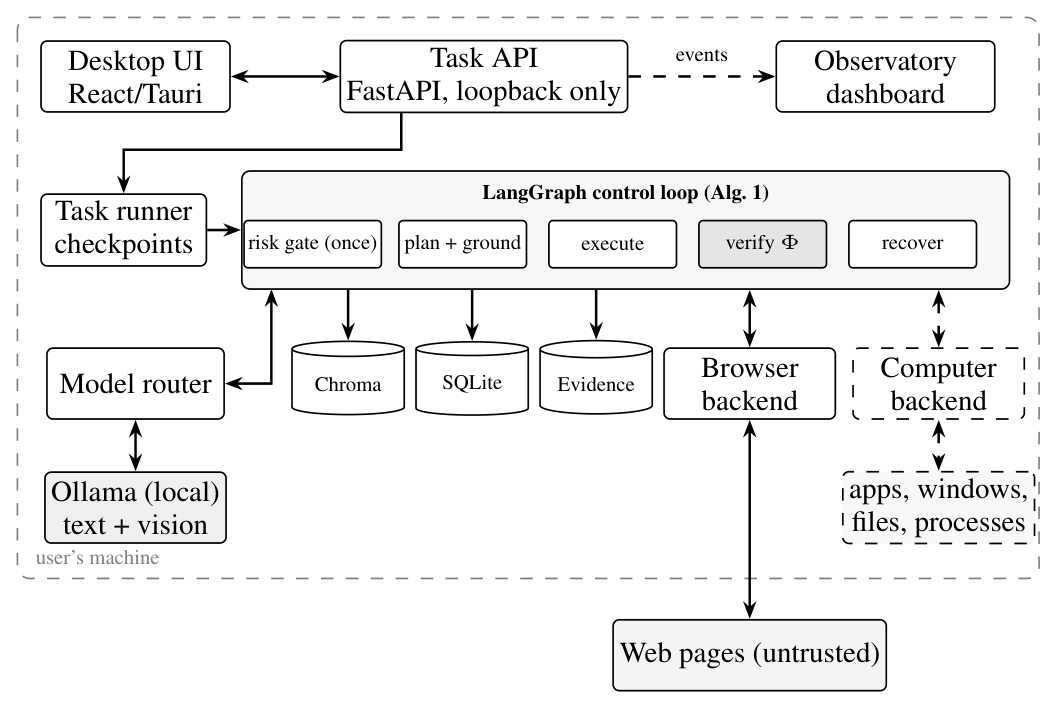
\includegraphics[width=0.95\textwidth]{fig/architecture.png}
\caption{Architecture of Agentic Pilot: desktop client, loopback FastAPI service, LangGraph control loop with the completion gate, Playwright browser backend, local models and local stores}
\label{fig:arch}
\end{figure}

The control loop is a compiled LangGraph state machine with eleven nodes. A typed state record carries the intent, the plan and step index, the current observation, the planned action, the action history, retry and model-call counters and the status. Only the verification node can end a task as \textsc{Completed}, and only when the completion predicate $\Phi$ holds. Each observation lists up to 50 ranked interactable page elements with role, label, text and selectors, sanitised against prompt injection. Actions are navigate, click, type, key press, scroll and extract; typed text is read back from the page. For each task, an evidence directory holds before-and-after screenshots of each action, the latest DOM manifest, the verification and recovery records and the node trace.

\subsection{Stakeholders}
Table~\ref{tab:stake} lists the groups the design has to keep in mind and what each needs from the system.

\begin{table}[h]
\caption{Stakeholders of the case and what each needs}
\label{tab:stake}
\small\singlespacing
\begin{tabularx}{\textwidth}{|p{3.3cm}|L|L|}
\hline\hrow \textbf{Stakeholder} & \textbf{Role in the case} & \textbf{What they need from the system}\\\hline
End users & Type requests and approve risky actions & Tasks done correctly; an honest ``not done''; screens not sent off the machine\\\hline
Developer (the author) & Designed, built and evaluated the prototype & Reproducible runs and records that support each claim\\\hline
Guide and examiners & Supervise and assess the work & Claims that match the evidence; clear separation of measured and simulated results\\\hline
Model publishers & Release open-weight models (Qwen, DeepSeek) run through Ollama & Correct use within licence terms\\\hline
Website operators & Run the sites the agent visits & No CAPTCHA solving or bot-check evasion by the agent\\\hline
Regulators and the institution & Set rules on personal data and software & Personal data kept on the device; compliance with the DPDP Act, 2023\\\hline
\end{tabularx}
\end{table}

\section{Problem statement and research questions}

A conventional agent equates a successful action call with progress and lets its model decide when the task is over. The problem in this case is to design an agent that keeps its inference and records on the user's machine, separates \emph{action dispatch} from \emph{task completion}, reports completion only when the observed page supports it, and to measure what this achieves and costs without overclaiming.

The research paper states three gaps, each phrased so that it can be tested:
\begin{itemize}
\item \textbf{G1.} In-loop completion checks are rarely measured. Does a rule over observed state inside the loop withhold premature completions, and at what false-rejection cost, on held-out data?
\item \textbf{G2.} The contribution of each kind of evidence is unknown. Does removing a conjunct of the rule raise false completions?
\item \textbf{G3.} Locality claims of local agents are rarely checked. Does the agent's process contact any host other than the local machine?
\end{itemize}
Five hypotheses, H1 to H5, extend these questions to the whole agent: fewer false completions (H1), more reliable completion decisions (H2), the effect of memory (H3), the effect of the recovery engine (H4) and the time overhead of verification (H5). They are examined in a seeded simulation, because a full study with a language-model planner was outside the scope of this case.

\section{Objectives and scope of the study}

The objectives are:
\begin{itemize}
\item to describe the prototype, its stakeholders and its setting well enough for the design to be judged;
\item to review related work on reasoning-and-acting agents, web and computer-use agents, completion checking, memory, security and local inference;
\item to analyse the recorded evidence with suitable statistics, tracing every number to a run record;
\item to compare what theory predicts with what the system did; and
\item to recommend how the work should proceed, with alternatives, risks and measures of success.
\end{itemize}

The study covers the browser backend and its components: the completion gate, browser control, locality enforcement, memory retrieval, recovery classification and the end-to-end oracle. Task-level success of the full agent with a language-model planner, the desktop backend (designed but not implemented in the evaluated commit) and physical hardware are out of scope.

\section{Different viewpoints on the case}
Table~\ref{tab:views} summarises five viewpoints on the prototype.

\begin{table}[h]
\caption{Summary of viewpoints on the case}
\label{tab:views}
\small\singlespacing
\begin{tabularx}{\textwidth}{|p{2.2cm}|L|L|}
\hline\hrow \textbf{Viewpoint} & \textbf{Main concern} & \textbf{What the case shows}\\\hline
Technical & Does the gate catch premature claims, and at what cost? & Withholds 9 of 22 held-out unsatisfied states, rejects 1 of 20 satisfied; 27\,ms per decision\\\hline
User and business & Is the agent useful if it sometimes refuses? & An honest ``not done'' is cheaper than a false ``done''; the gate's checks cover only some phrasings\\\hline
Social & Does it reduce misplaced trust in AI agents? & Stored evidence lets a user see why a task was or was not reported complete\\\hline
Ethical & Is the evaluation honest about what was measured? & Every number carries an evidence class; simulated results are not presented as measurements\\\hline
Legal & Is personal data handled lawfully? & Screens and prompts stay on the machine by default, which supports data minimisation under the DPDP Act, 2023\\\hline
\end{tabularx}
\end{table}

\textbf{Technical viewpoint.} A completion claim is accepted only when every check that the request triggers agrees. The measured cost is a median of 26.8\,ms per decision and no model call.

\textbf{User viewpoint.} A refused claim sends the agent back to work or ends the task honestly as unfinished. The user loses some convenience but gains a report they can trust.

\textbf{Social and ethical viewpoint.} Agents that overstate success can mislead people into acting on work that was never done. The evidence records make each decision inspectable.

\textbf{Legal viewpoint.} India's Digital Personal Data Protection Act, 2023 asks that personal data be processed for a lawful purpose and kept to what is necessary. An agent whose model runs on the user's own machine avoids transferring screen contents to a third party by default.

\section{Organisation of the report}
Chapter~\ref{ch:lit} reviews sources and related work. Chapter~\ref{ch:analysis} analyses the evidence and its limits. Chapter~\ref{ch:theory} applies the underlying theory. Chapter~\ref{ch:insights} draws insights and recommends a way forward, and Chapter~\ref{ch:concl} concludes. The appendices hold code listings, configuration, data samples and the run records.

\chapter{Information Sources and Literature Review}
\label{ch:lit}

\section{Sources used}

The case uses two kinds of source, listed in Table~\ref{tab:sources}: primary records that the project produced while building and testing the system, and secondary sources such as papers, documentation and law. No interviews, surveys or field observations took place, and no human participants were involved. The primary evidence is system evidence: run records, test logs, configuration, source code and saved outputs. Every number can be recomputed from files in the repository.

\begin{table}[h]
\caption{Sources used in the case study}
\label{tab:sources}
\small\singlespacing
\begin{tabularx}{\textwidth}{|p{1.7cm}|L|L|}
\hline\hrow \textbf{Type} & \textbf{Source} & \textbf{What it contributed}\\\hline
Primary & Gate study records (\texttt{verification\_gate\_cases.csv}, 92 constructed states in three sets) & Decisions, oracle labels and latency of the completion gate\\\hline
Primary & Ablation records (\texttt{verification\_gate\_ablation.csv}) & Effect of removing each conjunct\\\hline
Primary & Component measurements (\texttt{m2\_latency.json}, \texttt{m3\_recovery.csv}, \texttt{m4\_memory.csv}) & Browser latencies, recovery classification, retrieval ranks\\\hline
Primary & Egress logs (\texttt{e2e\_egress\_rerun/}, 70 episodes) & Every socket connection of the agent's Python processes\\\hline
Primary & Oracle validation (\texttt{e2e\_oracle\_validation.csv}, 114 scripted trajectories) & Agreement of the end-to-end oracle with intended verdicts\\\hline
Primary & Test logs (\texttt{pytest\_revision.txt}) & 144 of 147 unit and integration tests passing\\\hline
Primary & Simulation code and outputs (\texttt{benchmarks/simulation}, seeds 101 and 202) & \textsc{synthetic} estimates for H1--H5 under stated assumptions\\\hline
Primary & Source code and configuration (\texttt{backend/}, commit \texttt{bf0a8a5}) & Implementation audit; code listings in Appendix~A\\\hline
Secondary & Conference and journal papers on agents, benchmarks, memory, security and statistics & Related work and methods (References)\\\hline
Secondary & Legal and policy text (DPDP Act, 2023) & Legal viewpoint on personal data\\\hline
\end{tabularx}
\end{table}

\section{Review of related work and similar cases}

\subsection{Reasoning-and-acting agents}
ReAct interleaves reasoning with tool actions~\cite{yao2023react}, building on chain-of-thought prompting~\cite{wei2022chain}. Toolformer learns when to call an API~\cite{schick2023toolformer}. Reflexion and RCI let the model critique and retry its own attempts~\cite{shinn2023reflexion,kim2023rci}, and Voyager accumulates skills that a model checks~\cite{wang2024voyager}. In all of these a model decides that the task is finished. Huang et al.\ found that intrinsic self-correction, without outside feedback, does not reliably improve reasoning~\cite{huang2024cannot}. This finding motivates a completion check that does not rely on the same model.

\subsection{Web and computer-use agents and benchmarks}
Mind2Web pairs a ranker over DOM elements with a language model~\cite{deng2023mind2web}. WebVoyager drives live websites from screenshots~\cite{he2024webvoyager}. SeeAct finds that grounding actions on the page is the main bottleneck~\cite{zheng2024seeact}, which Set-of-Mark prompting addresses~\cite{yang2023som}. WebArena, VisualWebArena and WorkArena evaluate agents on self-hosted or remote applications with functional checks~\cite{zhou2024webarena,koh2024visualwebarena,drouin2024workarena}. OSWorld and Windows Agent Arena do so in real operating systems~\cite{xie2024osworld,bonatti2024waa}. UFO, Agent S and AppAgent control desktop and mobile applications~\cite{zhang2025ufo,agashe2025agents,zhang2025appagent}, and CogAgent, SeeClick, UI-TARS and OmniParser ground actions in screenshots~\cite{hong2024cogagent,cheng2024seeclick,qin2025uitars,lu2024omniparser}. These works say little about when the agent itself may conclude that a task is done.

\subsection{Completion checking}
Benchmark checkers run after the episode has ended. WebVoyager evaluates trajectories with a multimodal judge~\cite{he2024webvoyager}. Pan et al.\ use model-based evaluators to judge and refine agents~\cite{pan2024autonomous}, and Sumyk and Kosovan evaluate a vision-language completion judge on macOS applications~\cite{sumyk2025done}. The gate in Agentic Pilot applies the older idea of execution monitoring from planning and robotics~\cite{fikes1972planex,pettersson2005execution} to an LLM agent's completion claims: a rule over the observed state, \emph{inside} the loop, whose inputs are recorded and whose errors are measured.

\subsection{Memory, security and local inference}
Retrieval-augmented generation (RAG)~\cite{lewis2020rag,reimers2019sbert}, Generative Agents and MemGPT~\cite{park2023generative,packer2023memgpt} manage memory for language models and agents. Indirect prompt injection hides instructions in content that the agent reads~\cite{greshake2023indirect}; systematic evaluations find current defences insufficient~\cite{liu2024formalizing}. InjecAgent, AgentDojo, ToolEmu and OS-Harm measure unsafe agent behaviour~\cite{zhan2024injecagent,debenedetti2024agentdojo,ruan2024toolemu,kuntz2025osharm}, and CaMeL separates trusted control flow from untrusted data~\cite{debenedetti2025camel}. Open-weight models such as Qwen2.5 and Qwen2-VL~\cite{yang2024qwen25,wang2024qwen2vl} are released in sizes that, with 4-bit quantisation~\cite{lin2024awq}, run on consumer hardware. Surveys list trustworthiness among the open problems of LLM agents~\cite{wang2024survey,xi2025rise}.

Table~\ref{tab:related} compares representative systems, using only what each paper reports.

\begin{table}[h]
\caption{Comparison of related work with the case, from what each paper reports}
\label{tab:related}
\scriptsize\singlespacing
\setlength{\tabcolsep}{3pt}
\begin{tabularx}{\textwidth}{|L|l|l|l|l|l|l|l|}
\hline\hrow \textbf{System} & \textbf{Env.} & \textbf{Exec.} & \textbf{Completion decided by} & \textbf{Evid.} & \textbf{Mem.} & \textbf{Deploy.} & \textbf{Eval.}\\\hline
ReAct~\cite{yao2023react} & Ws & A & model & N & N & H & E2E\\\hline
Reflexion~\cite{shinn2023reflexion} & Ws & A & model$^{a}$ & N & Y & H & E2E\\\hline
WebArena~\cite{zhou2024webarena} & Wr & B & benchmark & n.r. & N & H & E2E\\\hline
Mind2Web~\cite{deng2023mind2web} & Wr & B & n/a & P & N & L & Off\\\hline
WebVoyager~\cite{he2024webvoyager} & W & A & model; judge$^{b}$ & Y & N & H & E2E\\\hline
SeeAct~\cite{zheng2024seeact} & W, Wr & A & model & n.r. & N & P & E2E, Off\\\hline
OSWorld~\cite{xie2024osworld} & D & B & benchmark & n.r. & N & L & E2E\\\hline
UFO~\cite{zhang2025ufo} & D & A & model & n.r. & P & H & E2E\\\hline
AppAgent~\cite{zhang2025appagent} & Mo & A & model & n.r. & Y & H & E2E\\\hline
CogAgent~\cite{hong2024cogagent} & Wr, Mo & M & n/a & N & N & L & Off\\\hline
MemGPT~\cite{packer2023memgpt} & Ws & A & n/a & N & Y & H & E2E$^{e}$\\\hline
AgentDojo~\cite{debenedetti2024agentdojo} & Ws & B & benchmark & n.r. & N & L & E2E\\\hline
\textbf{Agentic Pilot (this case)} & Wr$^{c}$ & A & in-loop rule & Y & P$^{d}$ & L & C+S\\\hline
\end{tabularx}

\vspace{3pt}
\raggedright
Env.: W live websites, Wr self-hosted or cached pages, Ws simulated web, tool or text environment, D desktop OS, Mo mobile. Exec.: A agent, B benchmark, M model. Evid.: per-step state artefacts. Mem.: memory across steps or episodes. Deploy.: L open-weight models, H hosted only, P partly. Eval.: E2E end-to-end tasks, Off offline step prediction, C+S component tests and simulation. Y yes, P partial, N no, n.r.\ not reported.
$^{a}$An evaluator gives feedback between trials. $^{b}$Used for evaluation. $^{c}$Evaluated on constructed states and self-hosted sites; the backend targets live websites. $^{d}$Implemented; retrieval measured on 10 queries over a synthetic corpus. $^{e}$Document QA and conversation tasks.
\end{table}

\section{Gaps identified and how this case addresses them}

Table~\ref{tab:gaps} maps the gaps found in the literature to the response in this case.

\begin{table}[h]
\caption{Gaps in the literature and the case's response}
\label{tab:gaps}
\small\singlespacing
\begin{tabularx}{\textwidth}{|p{0.7cm}|L|L|}
\hline\hrow \textbf{Gap} & \textbf{What is missing} & \textbf{How this case responds}\\\hline
G1 & Agents' own completion decisions are model-based; checks over observed state inside the loop are rarely measured on held-out data & A rule-based gate $\Phi$ in the verification node, evaluated on 92 constructed states including a set frozen before testing\\\hline
G2 & The value of each kind of evidence is unknown & Per-conjunct ablation of $\Phi$ on design and held-out states\\\hline
G3 & ``Local'' agents rarely test whether data leaves the machine & Loopback-only endpoint enforcement and a logged egress test over 70 episodes\\\hline
-- & Memory and recovery are reported without their failure modes & Retrieval ranks and recovery classification measured on the real components\\\hline
\end{tabularx}
\end{table}

\section{Credibility and currency of the sources}

The secondary sources are peer-reviewed conference and journal papers from 2019 to 2026 at venues such as NeurIPS, ICLR, ICML, ACL, EMNLP, CVPR, IEEE S\&P and USENIX Security, together with the classic statistical papers on which the analysis relies~\cite{wilson1927probable,clopper1934use,mcnemar1947note,efron1979bootstrap}. Preprints are used only for model reports and tools (Qwen2.5, Qwen2-VL, MemGPT, OmniParser, UI-TARS, CaMeL, Set-of-Mark), where no peer-reviewed version exists. DOIs and venues were checked against the publishers' records.

The primary sources are credible in a narrower sense. They are complete and reproducible: an independent recomputation of about 120 printed quantities from the raw files, with code that imported nothing from the project's analysis scripts, found no numerical mismatch, and reruns of the simulation and table generators in fresh clones gave byte-identical outputs. Their weakness is who wrote them: the constructed states and their labels were written by the same AI assistant that designed the gate fixes, and no second person has relabelled them. Chapter~\ref{ch:analysis} returns to this.

\chapter{Case Analysis (Data and Evidence)}
\label{ch:analysis}

\section{Description of the data and evidence}

The case rests on two completed studies. The first is a set of component-level experiments on the implementation, run without a language model. The second is a seeded simulation that carries those measurements through the agent's control flow under stated assumptions. To keep the two apart, every number in this report belongs to one of six evidence classes (Table~\ref{tab:classes}).

\begin{table}[h]
\caption{Evidence classes used for every number in the report}
\label{tab:classes}
\small\singlespacing
\begin{tabularx}{\textwidth}{|p{2.6cm}|L|}
\hline\hrow \textbf{Class} & \textbf{Meaning}\\\hline
\textsc{actual} & Executed or measured on the implementation\\\hline
\textsc{synthetic} & Produced by the simulation; not a measurement of the agent\\\hline
\textsc{assumed} & An input value chosen by the authors\\\hline
\textsc{derived} & Computed from existing results\\\hline
\textsc{literature} & Taken from cited work\\\hline
\textsc{proposed} & Designed but not implemented, or not yet done\\\hline
\end{tabularx}
\end{table}

Table~\ref{tab:data} lists the data analysed. The gate study ran on 2026-10-04 in a Linux container (4-core Xeon at 2.1\,GHz, no GPU) with Python~3.11.15, Playwright~1.56.0, Chromium~141, LangGraph~1.2.12 and Chroma~1.5.9. The component latencies were measured on 2026-10-23 on a 2.8\,GHz container.

\begin{table}[h]
\caption{Data and evidence used in the analysis}
\label{tab:data}
\small\singlespacing
\begin{tabularx}{\textwidth}{|L|p{2.2cm}|L|}
\hline\hrow \textbf{Data set} & \textbf{Class} & \textbf{Size and content}\\\hline
Gate states: design, held-out 1, held-out 2 & \textsc{actual} & 38, 12 and 42 constructed states (goal, URL, served HTML, answer, oracle label)\\\hline
Ablation & \textsc{actual} & Each conjunct removed in turn on all 92 states\\\hline
Component latency & \textsc{actual} & 30 repetitions each of navigate, click, fill, DOM extraction, screenshot and $\Phi$ on self-hosted pages\\\hline
Recovery classification & \textsc{actual} & 6 failure messages through the real recovery engine\\\hline
Memory retrieval & \textsc{actual} (synthetic corpus) & 10 queries over 22 stored records\\\hline
Egress test & \textsc{actual} & 70 control-loop episodes, every socket connection logged\\\hline
Oracle validation & \textsc{actual} & 114 scripted trajectories\\\hline
Test suite & \textsc{actual} & 147 tests\\\hline
Simulation v2 & \textsc{synthetic} & 100 scenarios (seed 202), 1{,}000 Monte Carlo sets, sensitivity sweeps\\\hline
\end{tabularx}
\end{table}

\section{Method of analysis}

\subsection{The completion predicate}
The agent observes an environment state $s_t$ through an observation $\Omega(s_t)$: URL, title, element list and screenshot. A planner maps a goal $g$, a plan $P=(g_1,\dots,g_n)$ and the observation to an action $a_t$. Executing it returns a \emph{dispatch flag} $\alpha_t\in\{0,1\}$, which says only that the call returned without error. The agent may report completion only when a predicate holds on the state observed \emph{after} the action:
\begin{equation}
\Phi(g,s_{t+1},P,\sigma) = \bigwedge_{c\in C(g,P)} c(s_{t+1}) \;\wedge\; \pi(P) \;\wedge\; \neg\beta(s_{t+1},\sigma),
\label{eq:phi}
\end{equation}
where $C(g,P)$ is the set of postconditions implied by the goal and plan, $\pi(P)$ states that no plan step is pending, and $\beta$ is a blocking condition (a bot-check page, an unapproved high-risk action) with $\sigma$ the approval state. Dispatch does not imply completion: $\alpha_t=1\not\Rightarrow\Phi=1$.

In the implemented browser predicate, $\Phi$ is the conjunction of six checks (Table~\ref{tab:conj}), each instantiated only when its trigger words occur in the request, plus a pre-check for $\beta$ that halts the task as \textsc{Blocked}. Fig.~\ref{fig:verify} shows the decision path.

\begin{table}[h]
\caption{Conjuncts of the implemented completion predicate $\Phi$}
\label{tab:conj}
\small\singlespacing
\begin{tabularx}{\textwidth}{|p{0.8cm}|p{3.2cm}|L|}
\hline\hrow \textbf{Check} & \textbf{Name} & \textbf{Fails when}\\\hline
$E$ & Error state & Browser-error URL; error or ``not found'' title; bot-check URL or title; redirect to a sign-in page when the request named another URL\\\hline
$H$ & Search home & Still on a search engine's home page when a search, extraction or multi-step plan was requested\\\hline
$Q$ & Query & The results page does not carry the query quoted in the request\\\hline
$T$ & Typed text & The text the request asks to enter is not present in an input (exactly, if the request says ``exactly'')\\\hline
$X$ & Extraction & For extraction requests, no answer that mentions a content word of the request\\\hline
$R$ & Remaining steps & A multi-step plan still has a pending step and no structured extraction exists\\\hline
$\beta$ & Bot-check pre-check & A CAPTCHA or security-check page is detected; the task halts as \textsc{Blocked}\\\hline
\end{tabularx}
\end{table}

\begin{figure}[h]
\centering
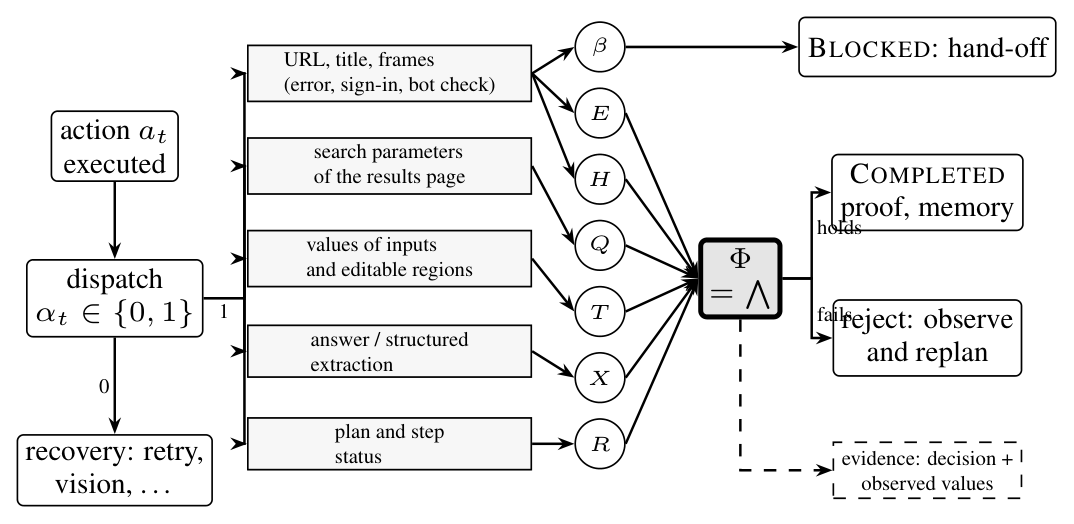
\includegraphics[width=0.9\textwidth]{fig/verification.png}
\caption{Decision path of the verification node: pre-check $\beta$, then the conjuncts of $\Phi$; only a passing state can end the task as \textsc{Completed}}
\label{fig:verify}
\end{figure}

\subsection{Metrics}
Let $\mathcal{T}$ be a set of end states, $\mathcal{T}_c$ those reported complete, and $\Phi^{\star}$ an oracle that shares no code with $\Phi$. With $N_{\mathrm{FC}}$ the states reported complete that the oracle marks unsatisfied, and $N_{\mathrm{FR}}$ the satisfied states not reported complete,
\begin{equation}
\mathrm{FCR} = \frac{N_{\mathrm{FC}}}{\lvert\mathcal{T}_c\rvert}, \qquad
\mathrm{FRR} = \frac{N_{\mathrm{FR}}}{\lvert\{\tau\in\mathcal{T}:\Phi^{\star}(\tau)=1\}\rvert}.
\label{eq:fcr}
\end{equation}
Because a dispatch-only rule reports every state complete, I also report the share of unsatisfied states that the gate withholds. Counts carry Wilson 95\% intervals~\cite{wilson1927probable}; paired comparisons on the same states use the exact McNemar test~\cite{mcnemar1947note} on decision correctness.

\subsection{Gate study design}
A state is a goal, a URL, an HTML document served through Playwright request interception, the agent's answer and plan state where relevant, and an oracle label. Every state ends with a dispatched action, so a dispatch-only rule accepts all of them. The \emph{design} set (38 states in six categories) was used to find the gate's defects and design fixes. \emph{Held-out~1} (12 states) was written after the fixes and not used to change them. \emph{Held-out~2} (42 states, 22 unsatisfied) was written to a fixed procedure with varied user phrasings and committed (\texttt{b9d5088}, SHA-256 recorded) before the gate was run on it. Each state is judged by the predicate called directly and by the real verification node with database, browser-pool and evidence I/O stubbed. Latency is the median of 20 repetitions after a warm-up.

\subsection{Simulation design}
The simulation draws 100 scenarios (seed 202), each with a task category and an outcome class that sets whether the goal is met. Detection and false-rejection rates are derived from the held-out gate states, latencies are resampled from the component measurements, and planner behaviour is assumed: chiefly the probability $\pi=0.65$ that a point at which the code evaluates $\Phi$ is reached while the task is unfinished, swept from 0.3 to 0.95. Monte Carlo replications regenerate 1{,}000 scenario sets with rates drawn from their Beta posteriors. The first model (v1) was committed before its scenarios were generated; an audit found four places where it contradicted the code, and the reported model, v2, was written after the v1 results were known. It is therefore post hoc, and the corrections moved results in favour of $\Phi$.

\section{Analysis and results}

\subsection{Completion gate (G1)}
Table~\ref{tab:gate} and Fig.~\ref{fig:gatechart} report the gate study (\textsc{actual}).

\begin{table}[h]
\caption{Completion gate on constructed states (\textsc{actual}). Withheld: unsatisfied states not reported complete. FR: satisfied states rejected. $p$: exact McNemar on paired correctness}
\label{tab:gate}
\small\singlespacing
\begin{tabularx}{\textwidth}{|L|c|c|c|c|}
\hline\hrow \textbf{Set and rule} & \textbf{Withheld} & \textbf{FR} & \textbf{$p$ vs dispatch-only} & \textbf{$p$ vs $E$ only}\\\hline
Design, before fixes (predicate) & 15/23 & 3/15 & -- & --\\\hline
Design, before fixes (live node, empty / verbose reasoning) & 14/23, 13/23 & -- & -- & --\\\hline
Design, after fixes$^{a}$ & 20/23 & 1/15 & -- & --\\\hline
Held-out 1 & 2/5 & 1/7 & 1.0 & 1.0\\\hline
Held-out 2 (frozen) & 9/22 & 1/20 & 0.021 & 0.070\\\hline
Pooled held-out & 11/27 & 2/27 & 0.022 & 0.11\\\hline
$E$ only, held-out 2 & 2/22 & 0/20 & -- & --\\\hline
Dispatch-only, any set & 0 & 0 & -- & --\\\hline
\end{tabularx}

\vspace{2pt}
\raggedright\footnotesize $^{a}$No test is reported on the design set, because the fixes were designed on it. Wilson 95\% intervals: design withheld 0.68--0.95; held-out 2 withheld 0.23--0.61, FR 0.01--0.24.
\end{table}

\begin{figure}[h]
\centering
\begin{tikzpicture}
\begin{axis}[ybar, bar width=14pt, width=0.78\textwidth, height=6.2cm,
  ymin=0, ymax=1.05, ylabel={Share}, ylabel style={font=\small},
  symbolic x coords={Design (before),Design (after),Held-out 1,Held-out 2},
  xtick=data, x tick label style={font=\small},
  legend style={at={(0.5,1.02)},anchor=south,legend columns=2,font=\small,draw=none},
  nodes near coords, every node near coord/.append style={font=\scriptsize,/pgf/number format/fixed,/pgf/number format/precision=2},
  enlarge x limits=0.18]
\addplot[fill=blue!55!black,draw=none] coordinates {(Design (before),0.652) (Design (after),0.870) (Held-out 1,0.400) (Held-out 2,0.409)};
\addplot[fill=orange!80!black,draw=none] coordinates {(Design (before),0.200) (Design (after),0.067) (Held-out 1,0.143) (Held-out 2,0.050)};
\legend{Unsatisfied states withheld, Satisfied states rejected}
\end{axis}
\end{tikzpicture}
\caption{Share of unsatisfied states withheld and of satisfied states rejected by the gate on each set (\textsc{actual}; counts in Table~\ref{tab:gate})}
\label{fig:gatechart}
\end{figure}

On the code before the fixes, the pre-check and $\Phi$ withheld 15 of the 23 unsatisfied design states and rejected 3 of the 15 satisfied ones. Inside the live verification node they withheld only 14 or 13, because the node let a premature \texttt{complete} action mark a pending step done and took the planner's reasoning for an answer. After the fixes all three modes agree on every state of every set. On the design states the gate withholds 20 of 23 and rejects 1 of 15, correcting 7 states relative to the earlier gate without breaking any.

The held-out sets give a less optimistic estimate. On held-out~2, frozen before testing, the gate withholds 9 of 22 unsatisfied states (0.41) and rejects 1 of 20 satisfied ones (0.05). It is correct alone on 9 states and wrong alone on 1, so it is correct on significantly more held-out states than a dispatch-only rule (exact McNemar $p=0.021$; pooled with held-out~1, 11 against 2, $p=0.022$). Against the stronger baseline of a detector that applies only the error check $E$, which withholds 2 of 22 and rejects none, the gate is correct alone on 7 states and wrong alone on 1 ($p=0.070$; pooled $p=0.11$). On new phrasings, then, the evidence that the checks beyond $E$ add accuracy is suggestive but not significant.

The misses follow from the rules. The answer check $X$ fires only on words such as ``extract'', so requests phrased ``tell me'' or ``what year'' are not checked; when it fires it accepts any answer that repeats a goal term. None of the 5 unsatisfied extraction states in held-out~2 is withheld. Unparsed text-entry phrasings, unfamiliar error titles and an add-to-cart click that added nothing also pass. The one false rejection is a page that merely mentions reCAPTCHA. The answer to G1 is a qualified yes.

\subsection{Contribution of each conjunct (G2)}
Table~\ref{tab:abl} gives the ablation (\textsc{actual}). Removing one check at a time raises false completions on the design states, most for the error check $E$ (3 to 8) and the search-home check $H$ (3 to 7), but changes at most three held-out decisions, and removing $Q$ or $X$ changes none. These checks rarely fire on phrasings they were not written for, so the gate's coverage, more than the strength of any single check, limits it. With at most five discordant states, the smallest attainable $p$ is 0.063, so the ablation is descriptive.

\begin{table}[h]
\caption{Per-conjunct ablation on the design states (\textsc{actual}): false completions (of 23) and false rejections (of 15)}
\label{tab:abl}
\small\singlespacing
\begin{tabular}{|l|c|c|c|c|c|c|c|c|}
\hline\hrow \textbf{Configuration} & \textbf{Full} & \textbf{$-E$} & \textbf{$-H$} & \textbf{$-Q$} & \textbf{$-T$} & \textbf{$-X$} & \textbf{$-R$} & \textbf{$-\beta$}\\\hline
False completions & 3 & 8 & 7 & 4 & 6 & 6 & 4 & 5\\\hline
False rejections & 1 & 1 & 1 & 1 & 1 & 0 & 1 & 1\\\hline
\end{tabular}
\end{table}

\subsection{Overhead}
$\Phi$ makes no model call and no browser action; it reads the page through the browser protocol. Over the 83 decisions that evaluate $\Phi$, the median latency was 26.8\,ms (90th percentile 29.5\,ms, 95th 30.3\,ms, maximum 34.6\,ms), and decisions stopped by the pre-check took at most 13.4\,ms. Table~\ref{tab:lat} puts this beside the other browser operations, measured on self-hosted pages, where $\Phi$ alone took 5.2\,ms.

\begin{table}[h]
\caption{Component latencies on self-hosted pages, 30 repetitions each (\textsc{actual}, 2.8\,GHz container)}
\label{tab:lat}
\small\singlespacing
\begin{tabular}{|l|c|c|}
\hline\hrow \textbf{Operation} & \textbf{Median (ms)} & \textbf{95th percentile (ms)}\\\hline
Navigate & 17.1 & 24.9\\\hline
Click & 65.2 & 106.2\\\hline
Fill text & 12.5 & 17.4\\\hline
DOM extraction & 76.4 & 105.6\\\hline
Screenshot & 61.3 & 93.6\\\hline
Predicate $\Phi$ & 5.2 & 6.9\\\hline
\end{tabular}
\end{table}

\subsection{Locality (G3)}
I ran 70 agent episodes (10 development tasks under 7 configurations, six with memory) through the real control loop and Chromium against local sites, with a scripted stand-in for the Ollama API on 127.0.0.1. Every \texttt{socket.connect} and \texttt{connect\_ex} call in the harness's eight Python processes was logged. All 555 connection attempts went to the stand-in on 127.0.0.1, and every page request that Playwright reported named host 127.0.0.1. A rerun on the clean commit \texttt{7133301} (agent code identical to \texttt{bf0a8a5}) gave the same result. Memory retrieval returned records in 54 of the 60 memory-enabled episodes. The stand-in performs no inference, and UDP, DNS lookups, the Playwright driver, Chromium and the model server were not instrumented; the result covers the agent's Python processes.

In addition, the model client refuses any endpoint whose host is not a loopback address or a \texttt{localhost} name, before connecting, unless the user sets \texttt{PILOT\_ALLOW\_REMOTE\_MODEL=true} (Listing~\ref{lst:locality}). Unit tests confirm that a remote model address is refused and that Chroma telemetry is off.

\subsection{Memory and recovery}
Memory retrieval was measured on 10 queries over 22 stored records (a synthetic corpus), 9 of which had a relevant record: precision at 3 was 0.52, the largest value attainable on this corpus; recall at 3 was 1.00; and the mean reciprocal rank was 0.93. In 3 of 10 queries, however, the top-ranked record was irrelevant or retrieval failed, because retrieval has no relevance threshold.

The recovery engine classified 6 failure messages and assigned the strategy sequence shown in Table~\ref{tab:rec}. A missing confirmation, where the task ended without its goal being met, was classified as \emph{unknown} and given the generic sequence; the engine does not recognise it.

\begin{table}[h]
\caption{Recovery classification of six failure messages by the real recovery engine (\textsc{actual})}
\label{tab:rec}
\small\singlespacing
\begin{tabularx}{\textwidth}{|p{3.2cm}|p{3.2cm}|L|}
\hline\hrow \textbf{Failure mode} & \textbf{Classified as} & \textbf{Strategy by retry count 0--5 (then exhausted)}\\\hline
Navigation failure & transient & retry, retry, alt.\ selector $\times2$, vision fallback $\times2$\\\hline
Timeout & transient & retry, retry, alt.\ selector $\times2$, vision fallback $\times2$\\\hline
Missing element & element not found & retry, retry, alt.\ selector $\times2$, vision fallback $\times2$\\\hline
Invalid submission & verification failed & retry, retry, replan $\times4$\\\hline
Unexpected state & vision needed & vision fallback $\times6$\\\hline
Missing confirmation & unknown & retry, retry, alt.\ selector $\times2$, vision fallback $\times2$\\\hline
\end{tabularx}
\end{table}

\subsection{Oracle validity and tests}
The end-to-end oracle agreed with the intended verdict on all 114 scripted trajectories. The informative cases are 35 correct solutions (no false negative) and 34 near misses (no false positive); the rest are negative by construction. This bounds errors only on anticipated behaviours. Of the 147 tests in the suite, 144 pass; the 3 failures need live websites or a running model.

\subsection{Simulation results (H1--H5)}
Table~\ref{tab:sim} summarises the seeded simulation. All its values are \textsc{synthetic} (simulation v2, revised post hoc): they follow from measured component behaviour and \textsc{assumed} planner behaviour, depend on those assumptions, and are not measurements of the agent.

\begin{table}[h]
\caption{Simulation results (\textsc{synthetic}, v2, post hoc; conditional on \textsc{assumed} inputs)}
\label{tab:sim}
\small\singlespacing
\begin{tabularx}{\textwidth}{|p{1.1cm}|L|L|}
\hline\hrow \textbf{Hyp.} & \textbf{Quantity} & \textbf{Result}\\\hline
H1 & False completions in 100 scenarios & 19 with $\Phi$ vs 28 without verification; paired reduction 0.11 per scenario [0.05, 0.18]; direction fixed by construction\\\hline
H2 & Correct decisions on 74 claims & 52 with $\Phi$ vs 46 accept-all; discordant 9/3, $p=0.15$; $\Phi$ better at $p<0.05$ in 42\% of Monte Carlo sets; not supported\\\hline
-- & Tasks achieved and reported & 44 with $\Phi$ vs 46 without verification\\\hline
H3 & Repeated workflows succeeding (of 44) & 19 without memory, 19 with memory, 20 with a proposed relevance filter\\\hline
H4 & Recoverable failures recovered (of 93) & 51 inline retries only, 68 with the engine, 87 with proposed evidence-guided recovery (by assumption)\\\hline
H5 & Mean episode time & $+2.6\%$ with $\Phi$; $+14\%$ with a model self-check\\\hline
\end{tabularx}
\end{table}

Two of the three false rejections by $\Phi$ in the simulation come from scenarios with missing evidence, which $\Phi$ rejects at an \textsc{assumed} rate of 0.8, whereas the measured false-rejection rate is 0 of 24. Fig.~\ref{fig:sens} shows the sensitivity to the unmeasured premature-claim rate $\pi$: the false completion rate is 0.14 with $\Phi$ against 0.21 without verification at $\pi=0.3$, and 0.32 against 0.45 at $\pi=0.95$, while the false rejection rate stays near 0.14 against 0.08.

\begin{figure}[h]
\centering
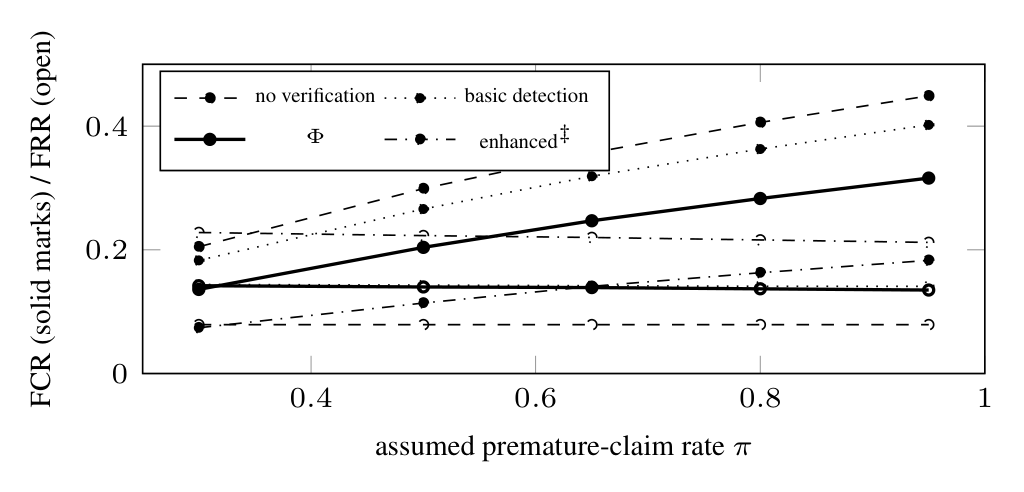
\includegraphics[width=0.72\textwidth]{fig/sensitivity.png}
\caption{Sensitivity of false completion and false rejection rates to the premature-claim rate $\pi$ (\textsc{synthetic}; 300 scenario sets per point)}
\label{fig:sens}
\end{figure}

\section{Validation of findings}

The findings were checked in four ways.
\begin{enumerate}
\item \textbf{Independent recomputation.} About 120 printed quantities were recomputed from the raw files with code that imported nothing from the project's analysis scripts. No numerical mismatch was found.
\item \textbf{Reproducibility.} The simulation, the table generators, the statistics script and the document build were rerun in fresh clones; all outputs were byte-identical.
\item \textbf{Freezing.} Held-out~2 was committed with its SHA-256 hash before the gate was run on it, and the code it ran on added only default-off switches and logging to the frozen gate.
\item \textbf{Agreement across modes.} After the fixes, the predicate called directly and the live verification node with empty or verbose reasoning agreed on every state.
\end{enumerate}

\section{Limitations of the data}

\begin{itemize}
\item The gate states are constructed, not sampled from real use. The states and their oracle labels were written by the AI assistant that also designed the gate fixes, and no second person relabelled them, so no inter-annotator agreement exists.
\item The sets are small. With 22 unsatisfied held-out states, the interval on the withheld share runs from 0.23 to 0.61.
\item The design-set result (20 of 23) is optimistic, because the fixes were made on those states.
\item The egress test used a scripted stand-in model server and logged only the Python processes' TCP connections.
\item Memory retrieval was measured on a small synthetic corpus with loosely grouped relevance labels.
\item The simulation is post hoc and conditional on assumed planner behaviour, above all the premature-claim rate $\pi$.
\item Task-level success of the full agent with a language-model planner was not measured in this study. A harness for it is released (Section~\ref{sec:harness}).
\end{itemize}

\chapter{Application of Theoretical Knowledge}
\label{ch:theory}

\section{Theories, models, frameworks and algorithms relevant to the case}

\subsection{Execution monitoring}
Classical planning separates what a plan intends from what the world shows. PLANEX executed STRIPS plans while comparing each step's expected conditions with the observed state~\cite{fikes1972planex}, and later work on execution monitoring in robotics generalised this to detecting discrepancies at run time~\cite{pettersson2005execution}. The completion gate is a monitor of this kind: the request implies postconditions, and the agent may not declare success until they are observed.

\subsection{Reasoning-and-acting loops as state machines}
A ReAct-style agent~\cite{yao2023react} alternates reasoning, action and observation. Agentic Pilot makes this loop explicit as a finite state machine in LangGraph: eleven nodes, a typed state record, and routing functions that select the next node. Algorithm~1 (Fig.~\ref{fig:alg}) gives the loop. The machine has one accepting transition to \textsc{Completed}, guarded by $\Phi$, so the property ``no task is reported complete unless $\Phi$ held'' follows from the structure of the graph rather than from the model's behaviour.

\begin{figure}[h]
\centering
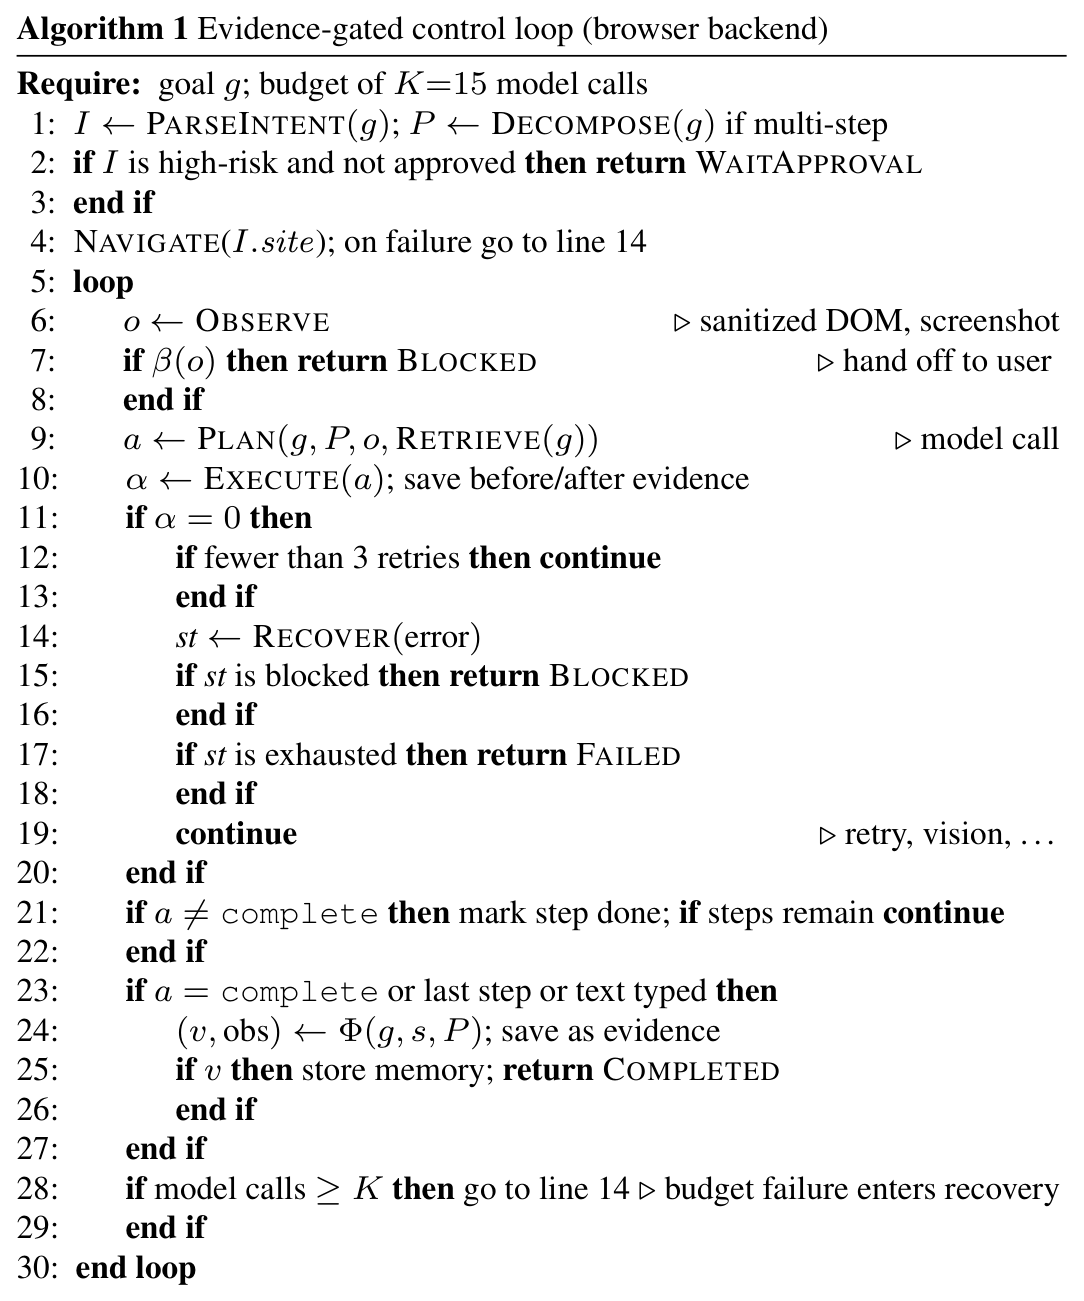
\includegraphics[width=0.85\textwidth]{fig/algorithm.png}
\caption{Algorithm 1: the evidence-gated control loop of Agentic Pilot}
\label{fig:alg}
\end{figure}

\subsection{Conjunctive decision rules and fail-closed design}
$\Phi$ is a conjunction of Boolean checks (Equation~\ref{eq:phi}). A conjunction fails closed: any check that fails, including one that cannot read the page, withholds completion. Adding a conjunct can only reduce false completions and can only raise false rejections, which is why the ablation in Chapter~\ref{ch:analysis} measures both. A rule with no tunable threshold has no ROC curve; its trade-off is characterised by removing conjuncts.

\subsection{Statistical inference for small samples}
The analysis uses methods suited to small counts. The Wilson score interval~\cite{wilson1927probable} behaves better than the normal approximation near 0 and 1; Clopper--Pearson intervals~\cite{clopper1934use} give an exact, conservative check. Paired decisions of two rules on the same states are compared with the exact McNemar test~\cite{mcnemar1947note}, which uses only the discordant pairs: with $b$ states where only the gate is correct and $c$ where only the baseline is correct,
\begin{equation}
p = \min\Bigl(1,\; 2\sum_{i=0}^{\min(b,c)} \binom{b+c}{i}\,2^{-(b+c)}\Bigr).
\end{equation}
For held-out~2 against dispatch-only, $b=9$ and $c=1$ give $p=0.021$. The same formula shows why some tests cannot succeed: with three discordant states the smallest attainable $p$ is 0.25.

\subsection{Monte Carlo simulation with Bayesian rate uncertainty}
The simulation propagates measured rates through the control flow. Each measured rate $k/n$ enters as a Beta posterior, and 1{,}000 scenario sets are regenerated with rates drawn from it, in the spirit of resampling methods~\cite{efron1979bootstrap}. Assumed planner parameters are swept rather than drawn, because no data constrain them.

\subsection{Retrieval-augmented memory}
Memory follows retrieval-augmented generation~\cite{lewis2020rag}: outcomes are stored in a local Chroma collection, embedded with Chroma's default sentence encoder~\cite{reimers2019sbert}, and the nearest records are inserted into later planning prompts. It is evaluated with standard ranking metrics, precision and recall at $k$ and mean reciprocal rank.

\subsection{Security principles}
Three principles apply. \emph{Privacy by design and data minimisation}: inference and records stay on the machine by default. \emph{Least privilege and human approval}: high-risk actions need the user's consent, and CAPTCHAs are left to the user. \emph{Treating page content as untrusted}: element text is sanitised against prompt injection~\cite{greshake2023indirect,liu2024formalizing}.

\section{Mapping of theory to the real-life situation}
Table~\ref{tab:map} maps each theory to where it appears in the case and what it predicted.

\begin{table}[h]
\caption{Mapping of theory to the case}
\label{tab:map}
\small\singlespacing
\begin{tabularx}{\textwidth}{|p{3.1cm}|L|L|}
\hline\hrow \textbf{Theory or model} & \textbf{Where it is used} & \textbf{What it predicts, and what happened}\\\hline
Execution monitoring & Verification node, $\Phi$ & Observed postconditions catch premature claims; held: 9 of 22 held-out claims withheld\\\hline
Finite state machine & LangGraph loop & Only one guarded path to \textsc{Completed}; held in every run\\\hline
Conjunctive, fail-closed rule & Six checks plus $\beta$ & Removing a check raises false completions; held on design states, little effect on held-out states\\\hline
Small-sample inference & Wilson intervals, McNemar & Wide intervals at $n\approx20$; held: 0.23--0.61\\\hline
Monte Carlo with Beta rates & Simulation v2 & Benefit depends on unmeasured inputs; shown by the $\pi$ sweep\\\hline
Retrieval-augmented memory & Chroma memory & Nearest records help planning only if relevant; 3 of 10 top-1 results were not\\\hline
Privacy by design & Loopback enforcement & No non-local connection from the Python processes; held in 70 episodes\\\hline
\end{tabularx}
\end{table}

\section{Course concepts applied}
Table~\ref{tab:course} lists the course concepts that the case applies.

\begin{table}[h]
\caption{Course concepts applied in the case, with justification}
\label{tab:course}
\small\singlespacing
\begin{tabularx}{\textwidth}{|p{3.6cm}|L|}
\hline\hrow \textbf{Concept} & \textbf{How it was applied}\\\hline
Case study method & A real system studied in its setting, with stakeholders, viewpoints and evidence\\\hline
Problem formulation & Gaps G1--G3 and hypotheses H1--H5 stated so that each can be tested\\\hline
Evidence and data analysis & Every number traced to a run record and an evidence class\\\hline
Experimental design & Design and held-out splits; a set frozen before testing; paired comparisons\\\hline
Validation and threats to validity & Recomputation, reproducibility runs, explicit limitations\\\hline
Decision analysis & Alternatives compared and a recommendation justified (Chapter~\ref{ch:insights})\\\hline
Professional ethics & Disclosure of AI assistance; no synthetic result presented as a measurement\\\hline
\end{tabularx}
\end{table}

\section{Where theory and practice differ, and why}

\textbf{Rules generalise less than they appear to.} In theory a postcondition check is exact. In practice, the postconditions are derived from the wording of the request, and new wordings escape them: the gate withheld 20 of 23 unsatisfied design states but 9 of 22 held-out ones. The checks are only as general as the trigger words they recognise.

\textbf{Dispatch is a weak signal even inside the code.} Before the fixes, the live verification node accepted fewer premature claims than the predicate alone, because it let a \texttt{complete} action mark a pending step done and treated the planner's reasoning as an answer. The theory of the predicate was right; the plumbing around it was not.

\textbf{Recovery is less diverse than its taxonomy.} The engine has seven failure types and four strategies, but only vision fallback changes behaviour; the others repeat ordinary planning. A missing confirmation, the failure the gate most often reveals, falls into ``unknown''.

\textbf{Locality is narrower than ``local''.} A loopback endpoint guarantees that prompts are sent to a server on the same machine, not that the server runs inference locally or that the browser itself contacts no other host.

\chapter{Insights, Decisions and Recommendations}
\label{ch:insights}

\section{Insights drawn from the analysis}

\begin{enumerate}
\item \textbf{Separating dispatch from completion pays off at low cost.} A rule over the observed page withheld 41\% of premature completions on held-out states, with one false rejection in 20 and a median decision time of 27\,ms with no model call.
\item \textbf{Coverage, not strength, limits the gate.} Each check works when it fires, but checks keyed to request wording fire rarely on new phrasings; extraction requests are the weakest category.
\item \textbf{The error check carries much of the measured benefit.} Against an $E$-only detector, the extra checks were correct on 7 more held-out states and wrong on 1 ($p=0.070$): promising, not yet established.
\item \textbf{Stored evidence exposed real defects.} Recording what each decision used revealed fixed extraction text, a node that trusted planner reasoning, an over-eager bot-check rule and inert features, all now fixed.
\item \textbf{Locality can be enforced and tested.} A loopback-only endpoint check and socket logging turned ``local'' from a claim into a tested property, within the stated scope.
\item \textbf{Memory and recovery need their own guards.} Retrieval without a relevance threshold returned irrelevant top records in 3 of 10 queries, and recovery does not recognise a missing confirmation.
\item \textbf{The agent-level benefit depends on the planner.} In simulation, how much the gate helps depends on how often the planner claims completion too early, which has not yet been measured.
\end{enumerate}

\section{Alternatives considered}
Table~\ref{tab:alt} compares four ways to decide when a task is complete.

\begin{table}[h]
\caption{Alternatives for deciding task completion}
\label{tab:alt}
\small\singlespacing
\begin{tabularx}{\textwidth}{|p{3.1cm}|L|L|}
\hline\hrow \textbf{Alternative} & \textbf{Strengths} & \textbf{Weaknesses}\\\hline
A. Accept the model's claim (dispatch-only) & Simplest; no false rejections & Every premature claim is reported as success\\\hline
B. Model self-check & Handles any phrasing & Intrinsic self-correction is unreliable~\cite{huang2024cannot}; costs a model call; $+14\%$ episode time in simulation\\\hline
C. Rule-based gate $\Phi$ (current) & Fast, inspectable, no model call; measured error rates & Coverage tied to request wording\\\hline
D. Rule gate plus model judge for unchecked requests & Keeps C's guarantees where rules fire; widens coverage & More complex; the judge's errors must be measured separately\\\hline
\end{tabularx}
\end{table}

\section{Recommended decision and its justification}

I recommend keeping the rule-based gate (alternative C) as the fail-closed authority on completion, and improving it in four ways:
\begin{enumerate}
\item widen the trigger vocabulary of the extraction check $X$ and the text-entry check $T$, and require answers to contain a value of the requested type rather than any goal term;
\item add a relevance threshold to memory retrieval, so that irrelevant records are not inserted into planning prompts;
\item add a missing-confirmation failure class to the recovery engine, with a strategy that re-reads the page before re-planning; and
\item consider alternative D only for requests on which no rule fires, with its own measured error rates.
\end{enumerate}
The justification is the evidence: the gate is correct on significantly more held-out states than accepting every claim, costs milliseconds, and its failures are specific enough to fix. A model self-check costs more and has no comparable measurement here.

\section{Implementation plan, risks and mitigation}

\begin{table}[h]
\caption{Implementation plan}
\label{tab:plan}
\small\singlespacing
\begin{tabularx}{\textwidth}{|p{1.6cm}|L|L|}
\hline\hrow \textbf{Phase} & \textbf{Work} & \textbf{Exit criterion}\\\hline
1 & Widen $X$ and $T$; write a new held-out set to a fixed procedure and freeze it before testing & Withheld share and false rejections reported with intervals on the new set\\\hline
2 & Relevance threshold for memory; missing-confirmation class for recovery & Retrieval and classification re-measured on the existing inputs\\\hline
3 & Run the released end-to-end harness with local models & Task success, false completions and false rejections per configuration\\\hline
4 & Independent relabelling of gate states by a second annotator & Agreement statistic (Cohen's $\kappa$~\cite{cohen1960coefficient}) reported\\\hline
\end{tabularx}
\end{table}

\begin{table}[h]
\caption{Main risks and their mitigation}
\label{tab:risk}
\small\singlespacing
\begin{tabularx}{\textwidth}{|p{4.2cm}|L|}
\hline\hrow \textbf{Risk} & \textbf{Mitigation}\\\hline
Wider triggers raise false rejections & Report false rejections beside every gain; keep a frozen held-out set\\\hline
Overfitting rules to test states & Design and held-out splits; freeze before running\\\hline
Small local models plan poorly & Report task success honestly; the gate still prevents false success reports\\\hline
Prompt injection through page text & Keep sanitisation; add injection tasks to the harness\\\hline
Remote endpoint set by mistake & Default refusal; the override must be set explicitly\\\hline
\end{tabularx}
\end{table}

\section{Expected impact and how it would be measured}

If adopted, the recommendations should reduce false success reports without a large rise in refusals. Impact would be measured with the released end-to-end harness (Section~\ref{sec:harness}): 40 tasks on five self-hosted sites with fictional content, at four difficulty tiers, under the full system, a no-check baseline and a self-verification baseline, three trials per task at temperature 0, scored by an oracle that reads only server-side records, the final URL and ground-truth facts. The success measures are task success rate, false completion rate and false rejection rate with intervals, and the median added time per decision. Wider adoption would also support data minimisation for users who automate tasks involving personal accounts.

\chapter{Conclusion and Future Scope}
\label{ch:concl}

\section{Summary of what was done and found}
This case study examined Agentic Pilot, a local browser agent that may report a task complete only when a rule over the observed page holds and that keeps its model traffic on the user's machine. The evidence came from the project's own records. On 42 held-out constructed states frozen before testing, the gate withheld 9 of 22 unsatisfied states and rejected 1 of 20 satisfied ones, which is significantly better than accepting every dispatched action ($p=0.021$) but not significantly better than an error-check-only detector ($p=0.070$). A decision takes a median of 27\,ms with no model call. In 70 episodes the agent's Python processes connected only to 127.0.0.1. Memory retrieval lacks a relevance threshold, and recovery misses absent confirmations. A seeded, post-hoc simulation shows that the gate's benefit to whole tasks depends on how often the planner claims completion too early.

\section{Lessons learnt}
\begin{itemize}
\item A successful action is not a finished task; making that distinction explicit in the control loop is cheap.
\item Rules written on known cases must be tested on cases written afterwards; the gap between 20 of 23 and 9 of 22 is the most useful number in this study.
\item Storing the evidence behind each decision finds bugs that tests miss.
\item Labelling every number with its evidence class keeps measured and simulated results apart, in writing as well as in analysis.
\end{itemize}

\section{Limitations of the study}
The states are constructed and were labelled by the AI assistant that designed the fixes, without a second annotator. The sets are small. The egress test used a stand-in model server and covered only the Python processes. The simulation is post hoc and depends on assumed planner behaviour. Task-level success of the full agent with a language-model planner is outside the scope of this study.

\section{Future scope}
\label{sec:harness}
\begin{itemize}
\item \textbf{End-to-end evaluation.} The released harness runs 40 tasks (10 development, 30 test) on five self-hosted sites under the full system, two baselines and one-factor ablations, with a validated oracle. Running it with local models would measure H1--H5 directly.
\item \textbf{Broader gate coverage.} Typed answer checks for extraction, more text-entry phrasings, and a measured model judge for requests that no rule covers.
\item \textbf{Memory and recovery.} A relevance threshold for retrieval and a missing-confirmation class with its own strategy.
\item \textbf{Desktop backend.} The same predicate form applies to desktop, file and process state, whose postconditions are typed and exact; in the evaluated commit the design exists but is not implemented. A later desktop automation subsystem on the \texttt{main} branch (Section~\ref{sec:cad}) has not been evaluated.
\item \textbf{Wider locality testing.} Instrument DNS, UDP, the browser and the model server.
\end{itemize}


\clearpage
\phantomsection
\addcontentsline{toc}{chapter}{REFERENCES}
\renewcommand{\bibname}{\centering REFERENCES}
{\singlespacing\small
\bibliographystyle{IEEEtran}
\bibliography{../paper/references}}

\clearpage
\appendix
\renewcommand{\thechapter}{\Alph{chapter}}
\titleformat{\chapter}[display]{\normalfont\bfseries\Large\centering}{APPENDIX \thechapter}{8pt}{\MakeUppercase}

\chapter{Code Listings}
All listings are taken verbatim from the evaluated branch.

\section{Loopback-only model endpoint (backend/security/locality.py)}
\lstinputlisting[caption={Locality enforcement},label={lst:locality}]{../backend/security/locality.py}

\section{Error, search-home and query checks of $\Phi$ (backend/verification/manager.py)}
\lstinputlisting[caption={Conjuncts $E$, $H$ and $Q$ of the completion predicate},label={lst:phi},firstline=221,lastline=287,firstnumber=221]{../backend/verification/manager.py}

\section{When the verification node evaluates $\Phi$ (backend/agent/nodes.py)}
\lstinputlisting[caption={Trigger for task-level verification},label={lst:trigger},firstline=1436,lastline=1445,firstnumber=1436]{../backend/agent/nodes.py}

\chapter{Configuration}
Settings are read from environment variables with the prefix \texttt{PILOT\_} (\texttt{backend/config.py}). Table~\ref{tab:config} lists those relevant to this study, with their defaults.

\begin{table}[h]
\caption{Configuration relevant to the study (defaults from backend/config.py)}
\label{tab:config}
\footnotesize\singlespacing
\begin{tabularx}{\textwidth}{|p{6.1cm}|p{2.9cm}|L|}
\hline\hrow \textbf{Variable} & \textbf{Default} & \textbf{Purpose}\\\hline
\texttt{PILOT\_OLLAMA\_BASE\_URL} & \texttt{127.0.0.1:11434} & Model server address\\\hline
\texttt{PILOT\_ALLOW\_REMOTE\_MODEL} & false & Allow a non-loopback endpoint\\\hline
\texttt{PILOT\_VERIFICATION\_MODE} & rule & \texttt{rule} ($\Phi$), \texttt{self} or \texttt{none}\\\hline
\texttt{PILOT\_VERIFICATION\_DISABLED\_CHECKS} & empty & Conjuncts removed for ablation\\\hline
\texttt{PILOT\_ENABLE\_RECOVERY / \_MEMORY} & true & Component switches\\\hline
\texttt{PILOT\_RECOVERY\_FIXED\_STRATEGY} & unset & Pin one recovery strategy\\\hline
\texttt{PILOT\_MAX\_RETRY\_COUNT} & 3 & Inline retries per task\\\hline
\texttt{PILOT\_MAX\_TASK\_DURATION\_MINUTES} & 5 & Wall-clock limit\\\hline
\texttt{PILOT\_LLM\_TEMPERATURE / \_SEED} & unset & Sampling for reproducible runs\\\hline
\texttt{PILOT\_MODEL\_REASONING} & \texttt{qwen2.5:7b} & Reasoning model\\\hline
\texttt{PILOT\_OLLAMA\_MODEL} & \texttt{qwen2.5:1.5b} & Default and fallback model\\\hline
\texttt{PILOT\_MODEL\_LIGHTWEIGHT} & \texttt{deepseek-r1:1.5b} & Light tasks\\\hline
\texttt{PILOT\_SERVER\_PORT} & 8765 & Loopback API port\\\hline
\end{tabularx}
\end{table}

\chapter{Data Samples}
Table~\ref{tab:samples} shows nine of the 42 held-out-2 states, every fifth row of \texttt{artifacts/results/verification\_gate\_cases.csv}.

\begin{table}[h]
\caption{Sample held-out-2 gate states and decisions (\textsc{actual})}
\label{tab:samples}
\scriptsize\singlespacing
\begin{tabularx}{\textwidth}{|p{0.6cm}|L|p{3.6cm}|p{0.6cm}|p{1.3cm}|}
\hline\hrow \textbf{Case} & \textbf{Goal} & \textbf{Oracle rationale} & \textbf{$\Phi^{\star}$} & \textbf{Gate}\\\hline
G1 & Look up `solar eclipse 2026' on Google & results for the requested query & 1 & completed\\\hline
G6 & Search Google for `electric cars' and show me the results & query typed but not submitted & 0 & rejected\\\hline
V5 & Take me to the contact page of example.org & contact page is open & 1 & completed\\\hline
B2 & Open https://en.wikipedia.org/wiki/Turing\_test & article about the topic & 1 & completed\\\hline
E1 & Go to notes.example.com and type `Buy milk' into the note & text present & 1 & completed\\\hline
E6 & Go to forms.example.com and type `Priya Raman' as the name & name filled & 1 & completed\\\hline
Xe & Find the capital of Australia on Wikipedia & wrong city & 0 & completed\\\hline
Xj & Extract the population of Tokyo from Wikipedia & answer lacks the population & 0 & completed\\\hline
M5 & Go to shop.example.com, open Laptops, then add the first laptop to the cart & add-to-cart dispatched but nothing added & 0 & completed\\\hline
\end{tabularx}
\end{table}

Xe, Xj and M5 are false completions of the kind discussed in Section~3.3.1: the extraction check does not fire on ``find'' and accepts any answer that repeats a goal term, and no check reads the cart.

\chapter{Run Records and Component Evidence}

\begin{table}[h]
\caption{Run records behind the results}
\label{tab:runs}
\scriptsize\singlespacing
\begin{tabularx}{\textwidth}{|p{2.6cm}|L|p{3.6cm}|p{1.6cm}|}
\hline\hrow \textbf{Result} & \textbf{File(s)} & \textbf{Command} & \textbf{Date / commit}\\\hline
Gate study, all sets & \texttt{verification\_gate\_cases.csv}, \texttt{gate\_stats.csv} & \texttt{verification\_gate\_study.py}; \texttt{gate\_stats.py} & 2026-10-04\\\hline
Held-out 2 freeze & \texttt{gate\_heldout2\_freeze.txt} & -- & \texttt{b9d5088}\\\hline
Gate before fixes & \texttt{verification\_gate\_cases\_before\_fixes.csv} & same, on old code & \texttt{08653e2}\\\hline
Ablation & \texttt{verification\_gate\_ablation.csv} & \texttt{verification\_gate\_study.py --ablation} & 2026-10-04\\\hline
Component latency, recovery, memory & \texttt{inputs/m2\_latency.json}, \texttt{m3\_recovery.csv}, \texttt{m4\_memory.csv} & \texttt{measure\_inputs.py} & 2026-10-23\\\hline
Egress & \texttt{e2e\_egress\_rerun/} & \texttt{run\_egress.py}; \texttt{summarize\_egress.py} & 2026-10-24, \texttt{7133301}\\\hline
Oracle validation & \texttt{e2e\_oracle\_validation.csv} & \texttt{python -m benchmarks.e2e.validate\_oracle} & --\\\hline
Tests & \texttt{pytest\_revision.txt} & \texttt{python -m pytest} & 2026-10-04\\\hline
Simulation & \texttt{out/heldout\_v2/results.json} & \texttt{simulate\_v2}; \texttt{make\_tables.py} & seeds 101, 202\\\hline
\end{tabularx}
\end{table}

\begin{table}[h]
\caption{Implementation status of the components}
\label{tab:status}
\small\singlespacing
\begin{tabularx}{\textwidth}{|L|p{6.2cm}|}
\hline\hrow \textbf{Component} & \textbf{Status}\\\hline
Completion predicate $\Phi$, bot-check halt & Implemented, evaluated (\textsc{actual})\\\hline
Browser control, DOM extraction & Implemented, evaluated (latency)\\\hline
Loopback endpoint enforcement & Implemented, tested (egress, unit tests)\\\hline
End-to-end oracle & Implemented, validated on 114 trajectories\\\hline
Recovery engine, memory & Implemented; measured and simulated\\\hline
Planner in the full loop, vision fallback, self-verification mode & Implemented, unit-tested, not separately evaluated\\\hline
Desktop backend, action gate, enhanced validation, guided recovery, memory filter & \textsc{proposed} in the evaluated commit; a later desktop subsystem on \texttt{main} is not evaluated\\\hline
\end{tabularx}
\end{table}


\end{document}
